\chapter{Introduction}
% -------------------------
%% QUOTE
\vspace*{\fill}
\epigraph{In all matters, before beginning,\\ a diligent preparation should be made.}%
{\textit{De Officiis (44 B.C.), I. 21.}\\ \textsc{Cisero}}
\clearpage{\thispagestyle{empty}\cleardoublepage}
%%
%% Body of the chapter
%%%%%%%%%%%%%%%%%%%%%%
\section{Motivation}

The surge in energy consumption levels is inevitable for modern societies. Their sustainability depends on it. The \usebibentry{EIA2017}{title} report \citeyearpar{EIA2017} published by the \usebibentry{EIA2017}{institution} projects a 28\% increase in world energy consumption between 2015 and 2040, assuming continuous improvement in known technologies based on current trends. As shown in Figure \ref{cht:energySources}, the consumption of ``petroleum and other liquid fuels" alone will grow by 18\%, which will account for 31\% of total world energy consumption in 2040.

\begin{figure}[b!]
    \centering
    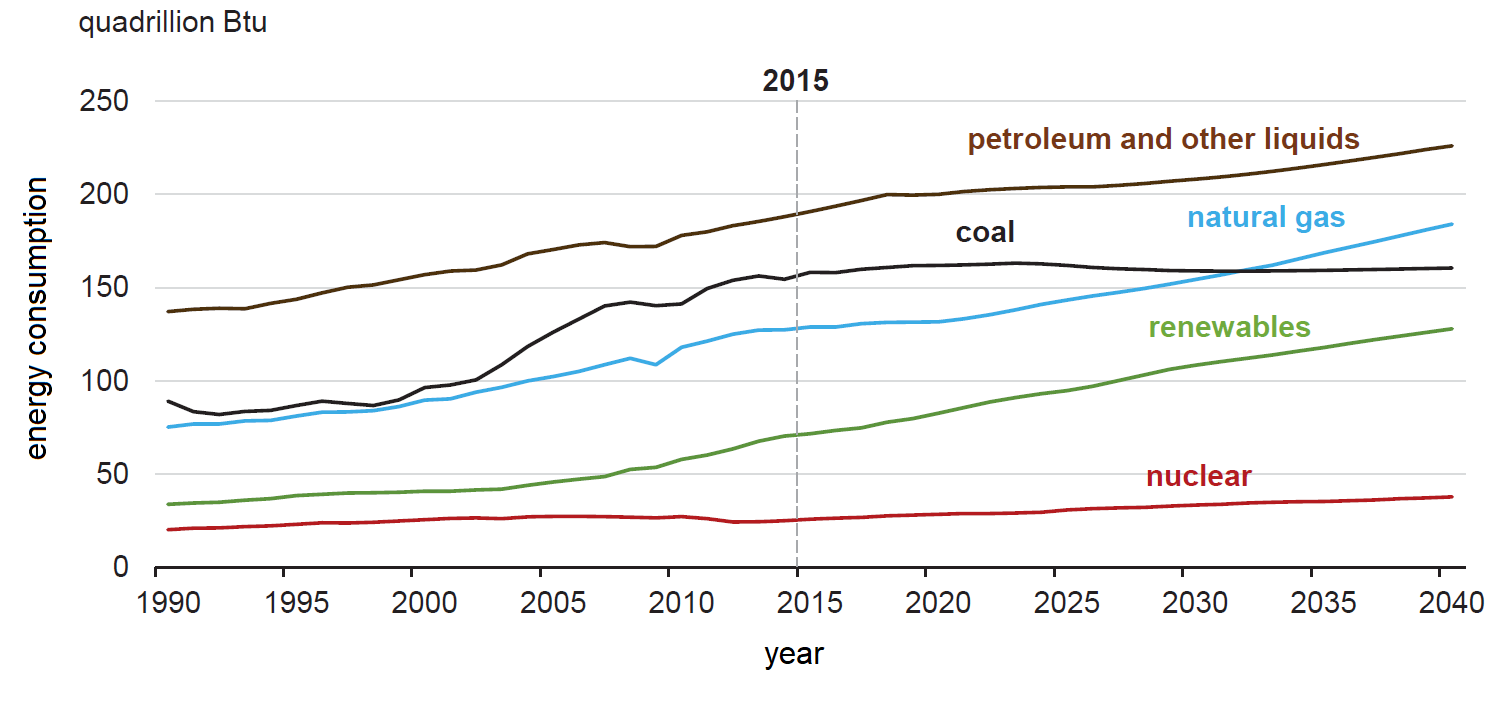
\includegraphics[width=\textwidth]{img/cht/chtEiaEnergy.png}
    \caption{World energy consumption by energy source \citep{EIA2017}}
    \label{cht:energySources}
\end{figure}

It is becoming more and more challenging to meet the ever-increasing demand for petroleum. Most of the existing major oilfields are already at a mature stage and the number of new significant discoveries per year is decreasing. Therefore, at this point in time, it is crucial to focus on methods of improving petroleum production from existing reservoirs. A big subset of such methods fall under the category of Enhanced Oil Recovery (EOR).

Challenges and technology gaps within EOR, \index{EOR!challenges} which need to be addressed in the coming research programs, have been identified in the OG21 strategy document on ``Exploration and Increased Recovery" \citep{OG21}: In particular, there is a need for more cost-efficient EOR chemicals, and to assure environmentally acceptable methods to avoid unwanted discharge to sea. Improved petroleum resource exploitation by EOR has also been given special attention in a report on increased recovery in the Norwegian Continental Shelf by the Norwegian Department of Oil and Energy \citep{Am2010}. There is therefore a clear need for increased competence in new technologies in the field of EOR. 

There has recently been an increasing interest in applying nanotechnology to EOR but still many topics are uncovered. Nanotechnology, \index{nanotechnology} which has mainly been developed in mechanical engineering, medicine and biological sciences, is expected to have a large potential for EOR applications. This technology has a wide range of applications relevant to EOR, from employing general concepts and principles of nanotechnology, to advanced reservoir monitoring using nano-sensors and nano-analysis, to more specific technologies which make up for the shortcomings in traditional EOR methods \citep{Fletcher2010, Ayatollahi2012, Cocuzza2011}. The latter includes tailoring chemical molecules for more efficient EOR, as well as smart and more effective delivery of EOR agents. Such technologies as efficient drug delivery in the human body may be applied to improve efficiency in chemical flooding.

This PhD work is part of the HyGreGel\index{HyGreGel|(} (Hybrid Green nano-Gels) project. The HyGreGel project addresses the need for more efficient water diversion techniques by improved in-depth placement of gelling chemicals to increase waterflood recovery and reduce unwanted water circulation in heterogeneous reservoirs. The project recognizes the environmental challenges using chemicals and emphasizes the development of green chemical systems for such applications.
%%%%%%%%%%%%%%%%%%%%%%
\section{Problem formulation}

Incremental recovery from water diversion is generally expected to be merely 2\% above standard water flooding \citep{OG21}. The main objective of HyGreGel is thus 
\begin{tcolorbox}
to improve incremental recovery from water diversion by developing and testing innovative hybrid (polymer + nanoparticle) gels.
\end{tcolorbox}
A thorough study of the effect of surface functionalities of the nanoparticles and their reactivity with the polymers will enable great improvements in controlling gel formation. This can be achieved by learning the scientific reasons behind the experimental results and understanding the kinetics of transport of nano-gels through porous media. Hence,  HyGreGel will contribute to making nanotechnology the next-generation EOR method.

The sub-goals of HyGreGel are:
\begin{enumerate}
    \item To study the effect of functional nanosized particles on the gel formation with polymers by cross-linking, and their transport through the oil reservoir.
    \item To synthetize and further develop  hybrid materials, both in terms of functionality and size.
    \item To investigate the reactivity of the nanosized particles with polymers, ensuring controlled gelling for several weeks and possibly months to assure in-depth placement of gels.
    \item To create basic knowledge on controlled release of encapsulated active components.
    \item To study the effect of real reservoir parameters such as temperature, pressure, brine salinity, and presence of crude oil on gel strength and gel stability and optimize the operational parameters.
    \item To study the integration of hybrid materials in industrial EOR.
\end{enumerate}

The results from HyGreGel will provide an understanding of how the nanoparticles affect the gel properties and their transport mechanism through the oil reservoir. They will also take major steps toward a robust design and manufacturing of hybrid gels. HyGreGel will keep the advantages of polymer materials (flexibility, processability and low cost) and make some improvement in EOR by integrating hybrid nanoparticles in the polymer. \index{HyGreGel|)}

%%%%%%%%%%%%%%%%%%%%%%
\section{Sub-projects}
The scientific work in the project was done through four sub-projects (SP). The research tasks and scientific methods for each of the SPs are described below.

\subsection*{SP1 --- Hybrid materials as sweeping efficiency modifier}
\addcontentsline{toc}{section}{\protect\numberline{}SP1 \quad Hybrid materials as sweeping efficiency modifier}%

SP1 was performed at the Department of Materials and Nanotechnology at SINTEF Industry (DMN). The approach is to use FunzioNano\texttrademark (FN)\index{FunzioNano} particles with functional groups having the ability to react with polymers causing cross-binding and gelling. Figure \ref{fig:sp1sp2} shows the gelation mechanism for SP1.

Hybrid materials based on FunzioNano are multifunctional nanoparticles which can provide significant benefit in EOR. FunzioNano with blocked functional groups can be used as a latent cross-linker for polymers which are made from renewable resources, e.g. cellulose based polymers. 

FunzioNano cross-linker and polymer are injected as a formulation at the same time. Hydrolysis within the requested time window leads to de-blocking of the functional groups and thereafter fast and efficient gelation by cross-linking of FunzioNano and polymer, e.g. through ionic bond formation between amine functionalities on FunzioNano and carboxylic functionalities on cellulose.

The time window for de-blocking FunzioNano can be adjusted by the type and the amount of hydrolysis catalyst. As an additional benefit cross-linked FunzioNano and polymer can provide a more hydrophobic gel than the components themselves. Motion of water could therefore be more efficiently hindered than motion of produced oil which would be suitable for partially blocking gels that can transport the remaining oil. FunzioNano can to a significant extent be manufactured from renewable resources. In case of un-desired spill, FunzioNano is degradable after being highly diluted with water. Computer modelling of the degradability of highly diluted FunzioNano was previously performed in collaboration with Université de Savoie, France \citep{Neyertz2012,Neyertz2013}.

\subsection*{SP2 --- Nanogels from polyelectrolyte complexes}
\addcontentsline{toc}{section}{\protect\numberline{}SP2 \quad Nanogels from polyelectrolyte complexes}

SP2 was performed at the Department of Exploration and Reservoir Technology (DER) and DMN at SINTEF Industry in co-operation with researchers at Texas A\&M University.

The task is to encapsulate active chemicals like cross-linkers by using polyelectrolyte complex \index{polyelectrolyte complexes} (PEC) nanoparticles to form a carrier which can be transported into a porous medium at relevant reservoir conditions. The hybrid materials developed in SP1 can be used as active chemicals to be encapsulated in PEC nanoparticles. 

Figure \ref{fig:sp1sp2} illustrates how hybrid systems contribute to form gel deep in the reservoir. The main challenge is to be able to control the release of the active components for correct location of the gel in the formation at conditions typical for North Sea reservoirs. The rheological properties (gelation rate, gel strength, stability) of the chemical gel system is studied in fluid bulk studies. The release of chemicals is analyzed, and factors which may influence the gelling rate is evaluated. Relevant pore scale mechanisms for the actual chemical system will be studied and analyzed.

\begin{figure}
    \centering
    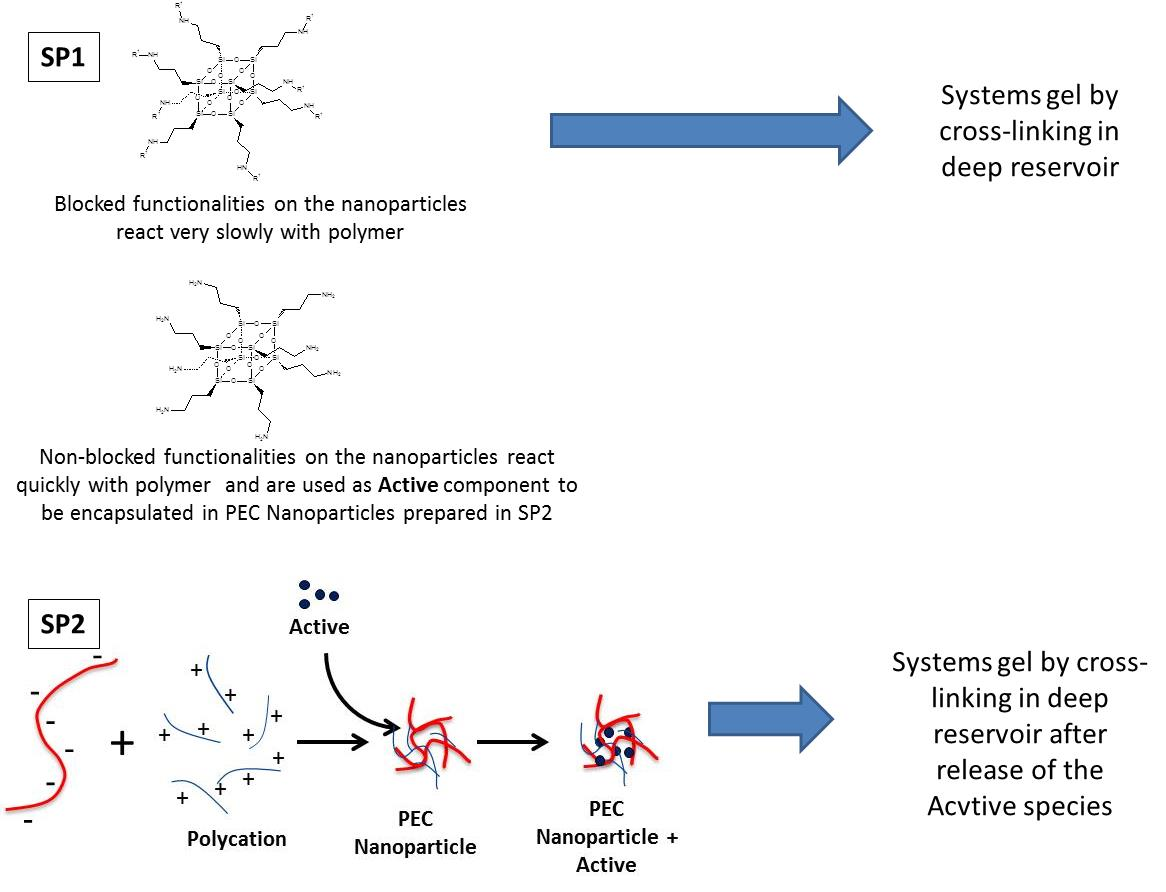
\includegraphics[width=\textwidth]{img/fig/sp1sp2.png}
    \caption{Gelation mechanisms in SP1 and SP2}
    \label{fig:sp1sp2}
\end{figure}

\subsection*{SP3 --- Transport of nanoparticles}
\addcontentsline{toc}{section}{\protect\numberline{}SP3 \quad Transport of nanoparticles}%
SP3 was performed at DER SINTEF Industry and the Department of Geoscience and Petroleum (IGP) NTNU.  
The constituents of the gelling chemicals should be easily transported together with the injected water without significant loss through the porous medium to the predetermined location where the gels are to be formed. The chemicals should withstand the actual reservoir conditions in the formation (temperature, pressure, salinity, presence of reservoir fluids, etc.), and the release of active chemicals should be controlled for correct in-depth placement of the gel structure. 

The placement of water diverting gels will be field specific depending on the reservoir geology and the actual performance of the water flood process. An in-depth gel treatment will require a thoroughly investigation and analysis of the reservoir water flood to define an optimal location of the gel. 

Flooding studies with injection of chemicals is performed in order to investigate transport properties of the chemical systems involved. The porous media selected for flooding studies need to be well characterized. The effect of water salinity on transport properties is studied by a set of core flooding studies (also in the presence of crude oil). In a field case the injected fluids are exposed to reservoir temperatures and pressures, and dedicated core flood studies will be performed to evaluate how temperature and pressure will affect the transport properties and gelling of the chemical system. Chemical analysis of the produced fluids is performed in order to characterize transport properties of the various components.

\subsection*{SP4 --- Numerical simulation of the hybrid gel/polymer interaction with water/oil/soil}
\addcontentsline{toc}{section}{\protect\numberline{}SP4 \quad Numerical simulation of the hybrid gel/polymer interaction with water/oil/soil}%

SP4 was performed as a co-operation between the DER and the Department of Industrial Process Technology (DIP) at SINTEF Industry. Two approaches were followed for modeling the gelation phenomenon. 

\textbf{Approach 1} --- \label{ref:sp4app1} A mathematical model of 1D two-phase flow with polymers and nanoparticles is developed, implemented and tested. The formulation includes tracking the age distribution of the nanoparticles in solution as well as the age distribution of absorbed nanoparticles. This means that at each position and time, the composition of the nanoparticles with respect to age and concentration are given. The age composition of the particles in solution in turn affects the nanoparticles ability to cross-link and form gel. Consequently, this formulation facilitates simulation of gel forming far away from the injection point. The simulator also includes the standard effects of polymer on water mobility, such as shear thinning, permeability reduction due to adsorbed polymer, and inaccessible pore space for polymers and nanoparticles.

The numerical formulation is first order upwind implicit for saturation, polymer, and nanoparticles. The tracking of the age distributions uses a novel explicit upstream, implicit downstream formulation giving accuracy (limited dispersion) and stability. The linear solver is also efficient and explicit (non-iterative), and the simulator uses an automatic time step control. 

\textbf{Approach 2} --- In a second approach, an alternative 1D model is established for the transport of the polymer and nanoparticles during flooding situations. Also in this model, the nanoparticles serve as cross-linking agent. A constitutive equation is formulated based on the gelation data for a given set of polymer concentrations, a given type of nanoparticles, and measured gelation times. In the model, a residence time for the nanoparticles is used to link the viscosity of the cross-linked polymer as the mixture is transported. The model has been used for simplified simulations of injection of time delayed gelling polymers to illustrate the functionality of the model and to carry out a sensitivity analysis.

%%%%%%%%%%%%%%%%%%%%%%
\section{Contributions and scope of the PhD work}

As mentioned earlier, this PhD work is a subset of the greater HyGreGel project. Therefore, it is important to clearly identify the scope of this work. A summary of the contributions are shown in Table \ref{tab:sp}. The primary contributions are as follows:

\begin{table}
\label{tab:sp} 
\small
\centering
\caption{Summary of contributions of the PhD work}
\begin{tabular}{p{0.38\textwidth} | c p{0.55\textwidth}} 
\toprule
\textbf{Sub-project} & \multicolumn{2}{l}{\textbf{Scope and contributions}}\\ 
\midrule 
%%
\multirow{2}{0.4\textwidth}{SP1: Hybrid materials as sweeping efficiency modifier} 
    & \tabitem & Test the reactivity of FN particles synthesized by DER \\
    & \tabitem & Select the most promising system for in situ gelling experiments\\
%% 
\midrule 
\multirow{2}{0.4\textwidth}{SP2: Nanogels from polyelectrolyte complexes} 
    & \tabitem & Prepare PEC samples according to Texas A\&M and new recipe \\
    & \tabitem & Age and test rheology of prepared samples \\
%%
\midrule 
\multirow{3}{0.4\textwidth}{SP3: Transport of nanoparticles} 
    & \tabitem & Run core flooding experiments with FN and polymer\\
    & \tabitem & Investigate transport of FN and polymer through porous media \\
    & \tabitem & Test possibility of mobility control using FN \\
%%
\midrule 
\multirow{3}{0.4\textwidth}{SP4: Numerical simulation of the hybrid gel/polymer interaction with water/oil/soil} 
    & \tabitem & Test numerical model with results from SP3\\
    & \tabitem & Run simulations with synthetic data sets \\
    & \tabitem & Test possibility of mobility control using FN \\
%%
\bottomrule
\end{tabular}
\end{table}

\begin{itemize}
    \item [\textbf{SP1}] The first gelation tests at DER with active FN particles and polymer revealed that it was difficult to form gels with cellulose based polymer but strong gels were formed with partially hydrolyzed polyacrylamide, HPAM. A low molecular weight HPAM was chosen as the base polymer for the following studies. DER followed two approaches in synthesizing FN-based particles. 
    
    Approach 1 --- The reactive groups of the FN particles were blocked to prevent instant cross binding with the polymer. Then, as a time dependent event, the blocked sites were activated by slow hydrolysis enabling cross-linking, viscosity increase and eventually gel formation.
    
    Approach 2 --- Only parts of the active sites were deactivated. DER found that by partially deactivation of the active sites the formation of gel was controlled to vary from several days to several months.
    
    {\color{blue} Contribution:} Both types of FN particles synthesized by DER were tested in bulk conditions. Their reactivity was tested by measuring viscosity and gel formation as a function of time at 80~\celsius~ in synthetic sea water at anaerobic conditions. Tested systems were kept in reaction vials and eventually the most promising system  was selected for \emph{in situ} gelling experiments.
    
    \item [\textbf{SP2}] Polyelectrolyte complexes \index{polyelectrolyte complexes} (PEC) can be made by mixing a polycation with a polyanion. By incorporating a cross-binder into the polyelectrolyte complex a delayed gel formation can be obtained. In the original PEC recipe \ce{Cr^3+} was used as cross-binder. As active FN particles are also polycations, Texas A\&M proposed that the original polycation was replaced by active FN. Initial tests carried out at Texas A\&M indicated that this could be a viable approach.
    
    {\color{blue} Contribution:} Samples of different basic systems were prepared for measurement of viscosity development with time. This included systems with only \ce{Cr^3+}-ions as cross-linker, systems based on the original Texas A\&M recipe and systems with active FN. Polymers of different molecular weight were used.
    
    Samples prepared according to published Texas A\&M technology showed that it was possible to delay gelation for in the order of 20 days when the sample was aged at 50~\celsius. At 80~\celsius~ the gelation was much faster, comparable to systems cross-linked with only \ce{Cr^3+}.
    
    When the PEC was modified by substituting the original polycation with active FN particles, and with use of polyvinylsulphonate as polyanion, delayed gelations in the order of 20 days and possibly longer was obtained for aging at 80~\celsius. The results indicate that the concept of making PECs with active FN as polycation may be viable. However, more experiments must be carried out to optimize the systems. Transport properties of PECs in porous media have not been investigated.
    
    Compared to the original Texas A\&M technology the new PEC reduces the number of components by one. This can possibly make the PEC more robust for transport in porous media where chromatographic separation of the constituents may occur. However, other factors may also govern the stability of PEC particles when transported in porous media.
    
    Retarded gelling obtained with a single cross-linker is possibly the best solution. The systems developed in SP1 appear to be promising. The requirement to retarded gelation will depend on how far into a reservoir a gel zone must be placed to obtain the desired water diversion. Then factors like initial viscosity, viscosity vs. time developments, shear tinning and allowable injection pressures become important for defining the properties of the chemical system.
    
    The polymer/polyelectrolyte solutions prepared in SP2 have been based on polymers with high molecular weights giving relatively high initial viscosities. The best system developed in SP1 was based on polymers that gave a significantly lower viscosity, although a higher polymer concentration was used. For practical applications (costs and logistics) it will be desirable to formulate a system which uses as little of chemicals as possible. After being injected and placed in a reservoir, the system must also cause an increase in viscosity enough to divert water. Thus, a further development work still will be needed to formulate an optimal system. 

    \item [\textbf{SP3}] {\color{blue} Contribution:} Several core flooding experiments were conducted where deactivated FN particles and polymer were injected both separately and in mixtures into two sets of sandstones, namely Berea and Bentheimer. The results indicate that polymer adsorption\index{adsorption}, polymer retention\index{retention} and inaccessible pore volume \index{inaccessible pore volume} (IPV) were generally reduced by the presence of nanoparticles. Adsorption, total retention and IPV were significantly higher in Berea compared to Bentheimer, for both polymer and nanoparticles. Adsorbed or otherwise retained polymer during injection was not released during following water floods, while the retained nanoparticles were partly released during subsequent water floods. Nanoparticles had negligible effect on rock permeability, while polymer significantly reduced rock permeability.
    
    The in situ gelling experiments incorporating the most promising system developed in SP1 demonstrated that gel was actually formed in the porous medium. As expected the gel strength increased with increased gelling time that was varied between 7 and 66 days. For the longest gelling time, a strong gel was formed. This gel essentially blocked water flow through the core for 9 days for an applied pressure gradient of 135 bar/m. Thereafter, injected synthetic sea water (SSW) flowed more readily, but still with a large pressure gradient across the core. The residual resistance factor \index{residual resistance factor} (RRF) after 75 pore volumes of injected SSW was still 3230. An injectivity problem of the nanoparticle/polymer solution was experienced. The cause of this problem has not been revealed, however.
    
    A certain type of deactivated FN particle was selected from SP1 to test whether it can improve oil recovery through mobility control during water flooding. The test was carried out in both water wet and neutral wet Berea cores. No improvements in the oil recovery were obtained.

    
    \item [\textbf{SP4}] {\color{blue} Contribution:} The numerical model in Approach 1 of SP4 (see page \pageref{ref:sp4app1}) was tested with results from the core flooding experiments in SP3 with deactivated FN particles and polymer. Simulations have also been run using a synthetic data set where polymer viscosity depends on polymer concentration and the concentration and age of the injected nanoparticles (the time passed since injection).
\end{itemize}

%%%%%%%%%%%%%%%%%%%%%%
\section{Thesis Structure}
The rest of this thesis is organized as follows:

\begin{description}
    \item [Chapter 2] presents background material for subsequent chapters. The chapter begins with an overview of EOR theory for context. 
    \item [Chapter 3] provides a literature review and state-of-the-art relevant to HyGreGel.
\end{description}